\label{lab:chapPET}
La Tomographie par \'Emission de Positons (TEP) est une modalité d'imagerie fonctionnelle utilisant la désintégration d'un traceur radioactif pour mettre en valeur les zones de forte activité métaboliques. Elle est principalement utilisée en imagerie cérébrale, oncologie et cardiologie.

\chapter{Principe Physique}

	\section{Généralités}

L'imagerie TEP permet de visualiser de manière indirecte des processus physiologiques survenant dans le corps du patient. Je vais présenter rapidement les évènements qui se produisent lors d'un examen, présentés dans la figure \ref{fig:schemaTEP}.


Pour cela, on lui injecte un ``traceur'' contenant une particule radioactive. Ce traceur est conçu de manière à se fixer sur les zones du corps que l'on souhaite imager. Pendant toute la durée de l'examen, les particules radioactives vont se désintégrer selon la loi de décroissance radioactive de la formule \ref{eq:loidecradioact}.

\begin{equation}
	dN = - \lambda N dt
	\label{eq:loidecradioact}
\end{equation}

$N$ représente le nombre le particules radioactives présentes dans le corps du patient. $dN$ représente la variation de ce nombre de particules (le nombre de désintégrations par $dt$) et $\lambda$ est une constante dépendant de l'élément radioactif.

Chaque désintégration d'un élément radioactif va déclencher l'émission d'une particule $\beta$, aussi appellée positon. En oncologie, on utilise le Fluor $^{18}F$ qui se désintégre en Oxygène $^{18}O$ en émettant le positon. Cette particule va parcourir quelques mm avant de s'annihiler avec un élection en émettant 2 photons dans deux directions opposées avec une énergie de 511 KeV.

Ce seront ces photons qui vont être détectés par l'imageur TEP pour reconstituer la position de la désintégration initiale. L'ensemble des ``Lignes de réponse'' (LDR) est utilisée pour reconstruire les images.

\begin{figure}
\centering
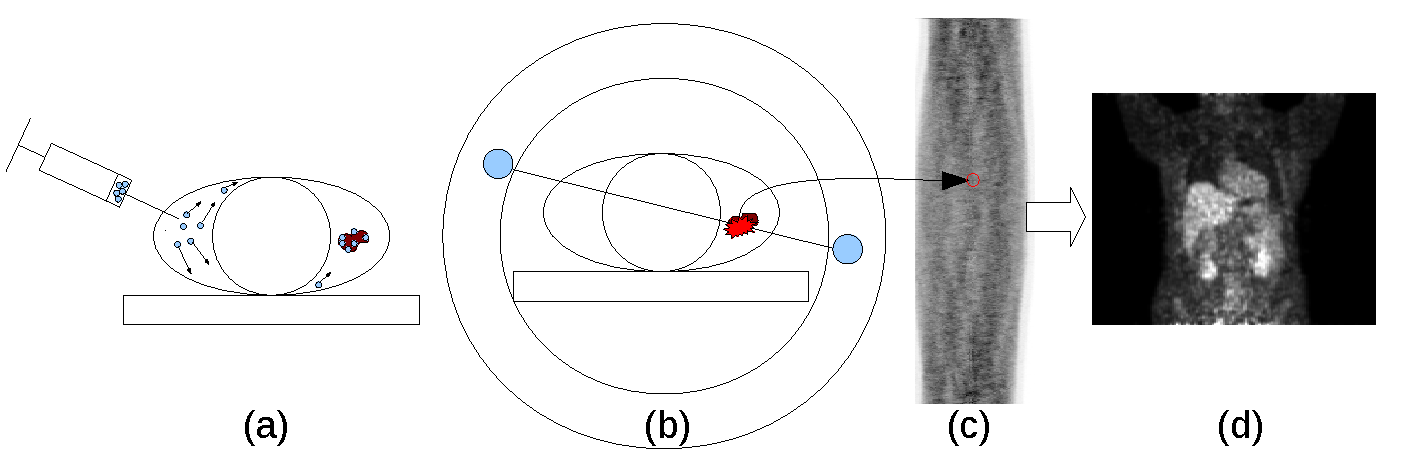
\includegraphics[width=16cm]{images/schemaTEP}
\caption[Présentation simplifiée de la TEP]{Processus d'un examen TEP : a) Injection du traceur radioactif, qui va se fixer préférentiellement sur les zones que l'on cherche à observer. b) Désintégration d'un atome radioactif du traceur, ici dans la zone à imager. Cela entraîne l'émission de deux photons dans deux directions opposées, qui seront détectés dans la couronne de capteurs. c) Tous les évènements détectés sont stockés dans la mémoire de la console, ici sous forme de sinogramme. d) L'image est reconstruite à la suite de l'acquisition pour former un volume 3D estimant la répartition du traceur dans l'organisme.}
\label{fig:schemaTEP}
\end{figure}

	\subsection{\'Emission des photons}

Nous allons maintenant détailler le processus qui déclenche l'émission des photons détectés par l'imageur, présenté dans la figure~\ref{fig:Langner2008ad}.

Les émetteurs de positons utilisés en TEP sont des isotopes radioactifs présentant un excès de charge positive, ou proton, dans leurs noyaux. Un processus de désintégration $\beta^+$, correspondant à la transformation d’un proton $p$ en un neutron $n$, leur permet de migrer vers un état stable. Cette désintégration résulte en l’émission d’un neutrino $\nu$ et d’un positron $e^+$ selon l’équation \ref{eq:desinteg}. Le positron est une particule de même masse que l’électron mais de charge opposée.

\begin{equation}
 p~\rightarrow~n + e^+ + \nu
\label{eq:desinteg}
\end{equation}

Le positon va alors s'annihiler avec un électron après un parcours de quelques millimètres en émettant deux photons de même énergie (511 keV) dans des directions opposées, comme indiqué dans l'équation~\ref{eq:annihilation}.

\begin{equation}
 e^+ + e^-~\rightarrow~\gamma + \gamma
\label{eq:annihilation}
\end{equation}

\begin{figure}
\centering
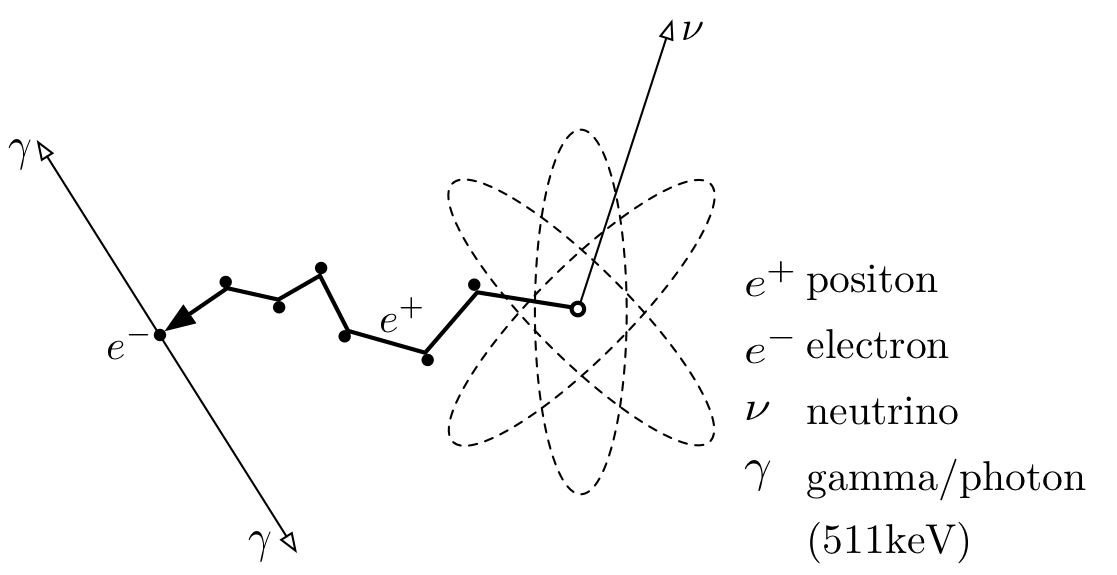
\includegraphics[width=12cm]{images/annihilation}
\caption[\'Emission des photons]{Emission des photons~\cite{Langner2008ad} : Le radiotraceur de désintègre en émettant un neutrino et un positron. Après un parcours de quelques mm dans les tissus, ce dernier s'annihile avec un électron. Cette réaction provoque la création de deux photons d'énergie 511 keV partant dans deux directions opposées.}
\label{fig:Langner2008ad}
\end{figure}



	\subsection{Détecteur}

Les détecteurs utilisés en TEP sont constitués d'un matériau photomultiplicateur placé devant un capteur. Chaque photon absorbé par le matériau photomultiplicateur va entraîner une réaction en chaîne qui qui va déclencher une émission lumineuse. Le capteur situé derrière va convertir cette émission lumineuse en charge électrique, qui sera transmise aux cartes de 

	\section{perturbation trajet du photon}

		\subsection{Diffusion}

		
		\subsection{Déviation}

La déviation apparaît lorsque le photon est absorbé par une particule puis ré-émis dans une autre direction. 	
		
		\subsection{Absorbtion}

L'absorbtion est un phénomène qui correspond à la suppression pure et simple du photon par les tissus our le matériel de l'imageur.

\chapter{Déroulement d'une acquisition}
	\section{2D / 3D}

Lors de l'appariment des photons, 


	\section{Format des données}
Les données acquises par une caméra TEP peuvent être stockées sous deux formes principales : Sinogramme et list-mode.
		\subsection{List-mode}

Ce format correspond à un enregistrement ``brut'' des données issues de l'électronique de la caméra.

Ce format de fichier est en fait un enregistrement séquentiel des évènements, dans leur ordre de détection. On peut enregistrer chaque détection indépendamment, ou encore uniquement les coïncidences. Les évènements sont datés, ce qui permet de conserver l'informations temporelles. 

Il existe plusieurs formats de fichiers pour le stockage de ces données, notamment le format LMF (List-Mode Format) développé pour le projet ClearPET et le format ROOT développé par le CERN. 

L'avantage de ces formats est qu'ils permettent de conserver les informations sur la dynamique de l'acquisition, mais aussi qu'ils permettent le stockage de métadonnées utiles en simulations, notamment le nombre de diffusions, ou de marquer les coincidences fortuites.

		\subsection{Sinogramme}

Le sinogramme est une image 
\chapter{Algorithmes de reconstruction}
	\section{Itératifs}
		\subsection{EM}
		\subsection{OSEM}
	\section{Analytiques}
